\chapter [Sensor Fusion and IMS]{Multisensor Data Fusion and Intersection Management Systems}

An intersection is a highly-dynamic scenario that can be monitored using a wide range of sensors. For this reason, an efficient and accurate fusion of the information is needed. This chapter is divided into two sections. In the first section a brief overview of multisensor data fusion is presented, remarking in different architectures proposed in the literature and different approaches used for laser and video data fusion.
The second section contains a short review on intelligent transportation systems and intersection management systems, including current research on this topic. Finally, there will be presented some projects that include fusion of laser and video data for intersection managing applications.

\section {Multisensor Data Fusion}

Data fusion, also referred as mutisensor data fusion, information fusion or sensor fusion, has received several definitions from different authors in the literature. For example, Joint Directors of Laboratories defined data fusion as "multi-level, multifaceted process handling the automatic detection, association, correlation, estimation, and combination of data and information from several sources"\cite{White1991}. Luo refers to multisensor fusion and integration as "synergistic combination of sensory data from multiple sensors to provide more reliable and accurate information"\cite{Luo2002} and "to achieve inferences that are not feasible from each individual sensor operating separately"\cite{Luo2011}. Elmenreich states that sensor fusion is "the combining of sensory data or data derived from sensory data such that the resulting information is in some sense better than would be possible when these sources were used individually"\cite{Elmenreich2007}. In \cite{Bostrom2007} there is a compilation of more definitions of information fusion and the author summarize in his own statement, i.e., "Information fusion is the study of efficient methods for automatically or semi-automatically transforming information from different sources and different points in time into a representation that provides effective support for human or automated decision making".  

% Elmenreich in [Elmenreich07]: Sensor fusion as "the combining of sensory data or data derived from sensory data such that the resulting information is in some sense better than would be possible when these sources were used individually"

%Khaleghi in [Kaleghi11]: "Multisensor data fusion is a technology to enable combining information from several sources in order to form a unified picture"

%White, JDL in [White91]: Data fusion as "multi- level, multifaceted process handling the automatic detection, association, correlation, estimation, and combination of data and information from several sources"

%Bostrom in [Bostrom07]: "Information fusion is the study of efficient methods for automatically or semi-automatically transforming information from different sources and different points in time into a representation that provides effective support for human or automated decision making"

%Luo refers to multisensor fusion and integration as "synergistic combination of sensory data from multiple sensors to provide more reliable and accurate information"\cite{Luo2002} and "to achieve inferences that are not feasible from each individual sensor operating separately"

All of previous definitions can be seen as a way to answer these three questions about data fusion:
\begin{itemize}
	\item {What is involved in data fusion?\\Combine, merge or integrate homogeneous or heterogeneous data.}
	\item {What is the aim of data fusion?\\Get a better representation of a process or the environment, infer underlying information, improve quality of the data.}
	\item {How to apply data fusion?\\Data fusion is a multi-level task, depending of the nature of the sensors, the final application and the environment.}
\end{itemize}

It is clear, now, that multisensor data fusion also is a multidisciplinary field, because information in a typical process, flows from sensors to applications, passing by stages of filtering, data enhancement and data extraction. Is for this that knowledge in a wide range of fields are required, e.g. signal processing, machine learning, probability and statistics, etc. Also, it would be pointless to try to define a general method, technique or architecture that fits the requirements of any system, for applying data fusion in it.


%\subsection{Overview}
\subsection{Architectures}

Although there is not a general rule of how to design or implement a sensor fusion system, many authors have proposed some architectures and guidelines for this task. One of the first proposals of fusion architecture, and probably one of the most widely used, is the JDL fusion model, originated from the US Joint Directors of Laboratories and described by Hall and Llinas in \cite{Hall1997} and \cite{Llinas1998}. The JDL fusion model was conceived to aid the developments of military applications and comprises 5 levels of data processing at which data fusion could be done. These levels and a database are connected by a bus (\ref{JDLmodel}), and are not meant to be execute sequentially and can also be executed concurrently.

\begin{figure}[ht!]
\centering
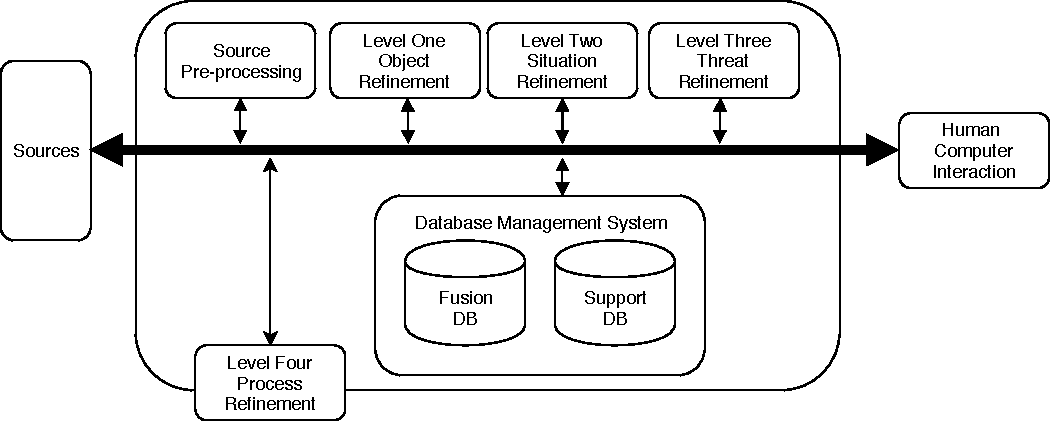
\includegraphics[scale=0.4]{fig/2/jdlmodel}
\caption{JDL fusion model. (from \cite{Hall1997}).}
\label{JDLmodel}
\end{figure}

\subsection{Laser and Video Data Fusion}

\section{Intersection Management Systems}
\subsection{Taxonomy}
\subsection{Intersection Management Systems and Multisensor Data Fusion}

\section{Conclusions}

Multisensor data fusion can be defined as the process of combine, merge or integrate data from homogeneous or heterogeneous set of sensors in order to get a better representation of a process, the environment or a situation, through the inference of underlying information and the improve of quality of data. Depending of the nature of the sensors and the source of information, fusion can be done in several manners, i.e., sensor-level fusion, feature-level fusion or decision-level fusion.
